%!TEX root = da-dev.tex

The study of distributed algorithms is closely related to graphs: we will interpret a computer network as a graph, and we will study computational problems related to this graph. In this section we will give a summary of the graph-theoretic concepts that we will use.

\section{Terminology}

A \emph{simple undirected graph} is a pair $G = (V,E)$, where $V$ is the set of \emph{nodes} (\emph{vertices}) and $E$ is the set of \emph{edges}. Each edge $e \in E$ is a 2-subset of nodes, that is, $e = \{u,v\}$ where $u \in V$, $v \in V$, and $u \ne v$. Unless otherwise mentioned, we assume that $V$ is a non-empty finite set; it follows that $E$ is a finite set. Usually, we will draw graphs using circles and lines\mydash each circle represents a node, and a line that connects two nodes represents an edge.


\subsection{Adjacency}

If $e = \{u,v\} \in E$, we say that node $u$ is \emph{adjacent} to $v$, nodes $u$ and $v$ are \emph{neighbours}, node $u$ is \emph{incident} to $e$, and edge $e$ is also \emph{incident} to $u$. If $e_1, e_2 \in E$, $e_1 \ne e_2$, and $e_1 \cap e_2 \ne \emptyset$ (i.e., $e_1$ and $e_2$ are distinct edges that share an endpoint), we say that $e_1$ is \emph{adjacent} to $e_2$.
\begin{figure}
    \centering
    \includegraphics[page=\PGraph]{figs.pdf}
    \caption{Node $u$ is adjacent to node $v$. Nodes $u$ and $v$ are incident to edge $e$. Edge $e_1$ is adjacent to edge $e_2$.}\label{fig:graph}
\end{figure}

The \emph{degree} of a node $v \in V$ in graph $G$ is \[
    \deg_G(v) = \bigl|\bigSet{ u \in V : \{u,v\} \in E }\bigr|.
\]
That is, $v$ has $\deg_G(v)$ neighbours; it is adjacent to $\deg_G(v)$ nodes and incident to $\deg_G(v)$ edges. A node $v \in V$ is \emph{isolated} if $\deg_G(v) = 0$. Graph $G$ is \emph{\Reg{k}} if $\deg_G(v) = k$ for each $v \in V$.


\subsection{Subgraphs}

Let $G = (V,E)$ and $H = (V_2,E_2)$ be two graphs. If $V_2 \subseteq V$ and $E_2 \subseteq E$, we say that $H$ is a \emph{subgraph} of $G$. If $V_2 = V$, we say that $H$ is a \emph{spanning subgraph} of $G$.

If $V_2 \subseteq V$ and $E_2 = \Set{ \{u,v\} \in E : u \in V_2,\ v \in V_2 }$, we say that $H = (V_2,E_2)$ is an \emph{induced subgraph}; more specifically, $H$ is the subgraph of $G$ induced by the set of nodes $V_2$.

If $E_2 \subseteq E$ and $V_2 = \bigcup E_2$, we say that $H$ is an \emph{edge-induced subgraph}; more specifically, $H$ is the subgraph of $G$ induced by the set of edges $E_2$.


\subsection{Walks}

\begin{figure}
    \centering
    \includegraphics[page=\PWalk]{figs.pdf}
    \caption{
        (a)~A walk of length~5 from $s$ to $t$.
        (b)~A non-backtracking walk.
        (c)~A path of length~4.
        (d)~A path of length~2; this is a shortest path and hence $\dist_G(s,t) = 2$.
    }\label{fig:walk}
\end{figure}

\begin{figure}
    \centering
    \includegraphics[page=\PCycle]{figs.pdf}
    \caption{
        (a)~A cycle of length~6.
        (b)~A cycle of length~3; this is a shortest cycle and hence the girth of the graph is~$3$.
    }\label{fig:cycle}
\end{figure}

A \emph{walk} of length $\ell$ from node $v_0$ to node $v_\ell$ is an alternating sequence \[w = (v_0, e_1, v_1, e_2, v_2, \dotsc, e_\ell, v_\ell)\] where $v_i \in V$, $e_i \in E$, and $e_i = \{ v_{i-1}, v_i \}$ for all $i$; see Figure~\ref{fig:walk}. The walk is \emph{empty} if $\ell = 0$. We say that walk~$w$ \emph{visits} the nodes $v_0, v_1, \dotsc, v_\ell$, and it \emph{traverses} the edges $e_1, e_2, \dotsc, e_\ell$. In general, a walk may visit the same node more than once and it may traverse the same edge more than once. A \emph{non-backtracking walk} does not traverse the same edge twice consecutively, that is, $e_{i-1} \ne e_i$ for all $i$. A \emph{path} is a walk that visits each node at most once, that is, $v_i \ne v_j$ for all $0 \le i < j \le \ell$. A walk is \emph{closed} if $v_0 = v_\ell$. A \emph{cycle} is a non-empty closed walk with $v_i \ne v_j$ and $e_i \ne e_j$ for all $1 \le i < j \le \ell$; see Figure~\ref{fig:cycle}. Note that the length of a cycle is at least~$3$.


\subsection{Connectivity and Distances}\label{ssec:graphs-conn}

For each graph $G = (V,E)$, we can define a relation $\leadsto$ on $V$ as follows: $u \leadsto v$ if there is a walk from $u$ to $v$. Clearly $\leadsto$ is an equivalence relation. Let $C \subseteq V$ be an equivalence class; the subgraph induced by $C$ is called a \emph{connected component} of $G$.

If $u$ and $v$ are in the same connected component, there is at least one \emph{shortest path} from $u$ to $v$, that is, a path from $u$ to $v$ of the smallest possible length. Let $\ell$ be the length of a shortest path from $u$ to $v$; we define that the \emph{distance} between $u$ and $v$ in $G$ is $\dist_G(u,v) = \ell$. If $u$ and $v$ are not in the same connected component, we define $\dist_G(u,v) = \infty$. Note that $\dist_G(u,u) = 0$ for any node $u$.

\begin{figure}
    \centering
    \includegraphics[page=\PNeighbourhood]{figs.pdf}
    \caption{Neighbourhoods.}\label{fig:neighbourhood}
\end{figure}
For each node $v$ and for a non-negative integer $r$, we define the \emph{radius-$r$ neighbourhood} of $v$ as follows (see Figure~\ref{fig:neighbourhood}):
\[
    \ball_G(v, r) = \Set{ u \in V : \dist_G(u,v) \le r }.
\]

A graph is \emph{connected} if it consists of one connected component. The \emph{diameter} of graph $G$, in notation $\diam(G)$, is the length of a longest shortest path, that is, the maximum of $\dist_G(u,v)$ over all $u, v \in V$; we have $\diam(G) = \infty$ if the graph is not connected.

The \emph{girth} of graph $G$ is the length of a shortest cycle in $G$. If the graph does not have any cycles, we define that the girth is $\infty$; in that case we say that $G$ is \emph{acyclic}.

A \emph{tree} is a connected, acyclic graph. If $T = (V,E)$ is a tree and $u,v \in V$, then there exists precisely one path from $u$ to $v$. An acyclic graph is also known as a \emph{forest}\mydash in a forest each connected component is a tree. A \emph{pseudotree} has at most one cycle, and in a \emph{pseudoforest} each connected component is a pseudotree.

A \emph{path graph} is a graph that consists of one path, and a \emph{cycle graph} is a graph that consists of one cycle. Put otherwise, a path graph is a tree in which all nodes have degree at most $2$, and a cycle graph is a \Reg{2} pseudotree. Note that any graph of maximum degree $2$ consists of disjoint paths and cycles, and any \Reg{2} graph consists of disjoint cycles.


\subsection{Isomorphism}

An \emph{isomorphism} from graph $G_1 = (V_1,E_1)$ to graph $G_2 = (V_2,E_2)$ is a bijection $f\colon V_1 \to V_2$ that preserves adjacency: $\{u,v\} \in E_1$ if and only if $\{f(u),f(v)\} \in E_2$. If an isomorphism from $G_1$ to $G_2$ exists, we say that $G_1$ and $G_2$ are isomorphic.

If $G_1$ and $G_2$ are isomorphic, they have the same structure; informally, $G_2$ can be constructed by renaming the nodes of $G_1$ and vice versa.


\section{Packing and Covering}\label{sec:packingcovering}

A subset of nodes $X \subseteq V$ is
\begin{enumerate}
    \item an \emph{independent set} if each edge has at most one endpoint in $X$, that is, $|e \cap X| \le 1$ for all $e \in E$,
    \item a \emph{vertex cover} if each edge has at least one endpoint in $X$, that is, $e \cap X \ne \emptyset$ for all $e \in E$,
    \item a \emph{dominating set} if each node $v \notin X$ has at least one neighbour in $X$, that is, $\ball_G(v,1) \cap X \ne \emptyset$ for all $v \in V$.
\end{enumerate}
A subset of edges $X \subseteq E$ is
\begin{enumerate}[resume]
    \item a \emph{matching} if each node has at most one incident edge in $X$, that is, $\{t,u\} \in X$ and $\{t,v\} \in X$ implies $u = v$,
    \item an \emph{edge cover} if each node has at least one incident edge in $X$, that is, $\bigcup X = V$,
    \item an \emph{edge dominating set} if each edge $e \notin X$ has at least one neighbour in $X$, that is, $e \cap \bigl(\bigcup X\bigr) \ne \emptyset$ for all $e \in E$.
\end{enumerate}
See Figure~\ref{fig:packingcovering} for illustrations.
\begin{figure}
    \centering
    \includegraphics[page=\PPackingCovering]{figs.pdf}
    \caption{Packing and covering problems; see Section~\ref{sec:packingcovering}.}\label{fig:packingcovering}
\end{figure}

Independent sets and matchings are examples of \emph{packing problems}\mydash intuitively, we have to ``pack'' elements into set $X$ while avoiding conflicts. Packing problems are \emph{maximisation problems}. Typically, it is trivial to find a feasible solution (for example, an empty set), but it is more challenging to find a large solution.

Vertex covers, edge covers, dominating sets, and edge dominating sets are examples of \emph{covering problems}\mydash intuitively, we have to find a set $X$ that ``covers'' the relevant parts of the graph. Covering problems are \emph{minimisation problems}. Typically, it is trivial to find a feasible solution if it exists (for example, the set of all nodes or all edges), but it is more challenging to find a small solution.

The following terms are commonly used in the context of maximisation problems; it is important not to confuse them:
\begin{enumerate}
    \item \textbf{\emph{maximal}}: a maximal solution is not a proper subset of another feasible solution,
    \item \textbf{\emph{maximum}}: a maximum solution is a solution of the largest possible cardinality.
\end{enumerate}
Similarly, in the context of minimisation problems, analogous terms are used:
\begin{enumerate}
    \item \textbf{\emph{minimal}}: a minimal solution is not a proper superset of another feasible solution,
    \item \textbf{\emph{minimum}}: a minimum solution is a solution of the smallest possible cardinality.
\end{enumerate}
Using this convention, we can define the terms \emph{maximal independent set}, \emph{maximum independent set}, \emph{maximal matching}, \emph{maximum matching}, \emph{minimal vertex cover}, \emph{minimum vertex cover}, etc.

For example, Figure~\ref{fig:packingcovering}a shows a maximal independent set: it is not possible to greedily extend the set by adding another element. However, it is not a maximum independent set: there exists an independent set of size $3$. Figure~\ref{fig:packingcovering}d shows a matching, but it is not a maximal matching, and therefore it is not a maximum matching either.

Typically, maximal and minimal solutions are easy to find\mydash you can apply a greedy algorithm. However, maximum and minimum solutions can be very difficult to find\mydash many of these problems are NP-hard optimisation problems.

A \emph{minimum maximal matching} is precisely what the name suggests: it is a maximal matching of the smallest possible cardinality. We can define a \emph{minimum maximal independent set}, etc., in an analogous manner.


\section{Labellings and Partitions}\label{sec:partitions}

We will often encounter functions of the form \[f\colon V \to \{1,2,\dotsc,k\}.\] There are two interpretations that are often helpful:
\begin{enumerate}[label=(\roman*)]
    \item Function $f$ assigns a \emph{label} $f(v)$ to each node $v \in V$. Depending on the context, the labels can be interpreted as colours, time slots, etc.
    \item Function $f$ is a \emph{partition} of $V$. More specifically, $f$ defines a partition $V = V_1 \cup V_2 \cup \dotsb \cup V_k$ where $V_i = f^{-1}(i) = \Set{ v \in V : f(v) = i }$.
\end{enumerate}
Similarly, we can study a function of the form \[f\colon E \to \{1,2,\dotsc,k\}\] and interpret it either as a labelling of edges or as a partition of~$E$.

Many graph problems are related to such functions. We say that a function $f\colon V \to \{1,2,\dotsc,k\}$ is
\begin{enumerate}
    \item a \emph{proper vertex colouring} if $f^{-1}(i)$ is an independent set for each~$i$,
    \item a \emph{weak colouring} if each non-isolated node $u$ has a neighbour $v$ with $f(u) \ne f(v)$,
    \item a \emph{domatic partition} if $f^{-1}(i)$ is a dominating set for each~$i$.
\end{enumerate}
A function $f\colon E \to \{1,2,\dotsc,k\}$ is
\begin{enumerate}[resume]
    \item a \emph{proper edge colouring} if $f^{-1}(i)$ is a matching for each~$i$,
    \item an \emph{edge domatic partition} if $f^{-1}(i)$ is an edge dominating set for each~$i$.
\end{enumerate}
See Figure~\ref{fig:partitions} for illustrations.
\begin{figure}
    \centering
    \includegraphics[page=\PPartitions]{figs.pdf}
    \caption{Partition problems; see Section~\ref{sec:partitions}.}\label{fig:partitions}
\end{figure}

Usually, the term \emph{colouring} refers to a proper vertex colouring, and the term \emph{edge colouring} refers to a proper edge colouring. The value of $k$ is the \emph{size} of the colouring or the \emph{number of colours}. We will use the term \emph{$k$-colouring} to refer to a proper vertex colouring with $k$ colours; the term \emph{$k$-edge colouring} is defined in an analogous manner.

A graph that admits a $2$-colouring is a \emph{bipartite graph}. Equivalently, a bipartite graph is a graph that does not have an odd cycle.

Graph colouring is typically interpreted as a minimisation problem. It is easy to find a proper vertex colouring or a proper edge colouring if we can use arbitrarily many colours; however, it is difficult to find an \emph{optimal} colouring that uses the smallest possible number of colours.

On the other hand, domatic partitions are a maximisation problem. It is trivial to find a domatic partition of size $1$; however, it is difficult to find an \emph{optimal} domatic partition with the largest possible number of disjoint dominating sets.


\section{Factors and Factorisations}

Let $G = (V,E)$ be a graph, let $X \subseteq E$ be a set of edges, and let $H = (U,X)$ be the subgraph of $G$ induced by $X$. We say that $X$ is a \emph{$d$-factor} of $G$ if $U = V$ and $\deg_H(v) = d$ for each $v \in V$.

Equivalently, $X$ is a $d$-factor if $X$ induces a spanning \Reg{d} subgraph of $G$. Put otherwise, $X$ is a $d$-factor if each node $v \in V$ is incident to exactly $d$ edges of $X$.

A function $f\colon E \to \{1,2,\dotsc,k\}$ is a \emph{\Fact{d}} of $G$ if $f^{-1}(i)$ is a $d$-factor for each $i$. See Figure~\ref{fig:factorisation} for examples.
\begin{figure}
    \centering
    \includegraphics[page=\PFactorisation]{figs.pdf}
    \caption{
        (a)~A \Fact{1} of a \Reg{3} graph.
        (b)~A \Fact{2} of a \Reg{4} graph.
    }\label{fig:factorisation}
\end{figure}

We make the following observations:
\begin{enumerate}
    \item A $1$-factor is a maximum matching. If a $1$-factor exists, a maximum matching is a $1$-factor.
    \item A \Fact{1} is an edge colouring.
    \item The subgraph induced by a $2$-factor consists of disjoint cycles.
\end{enumerate}
A $1$-factor is also known as a \emph{perfect matching}.


\section{Approximations}

So far we have encountered a number of maximisation problems and minimisation problems. More formally, the definition of a maximisation problem consists of two parts: a set of \emph{feasible solutions} $\calS$ and an \emph{objective function} $g\colon \calS \to \RR$. In a maximisation problem, the goal is to find a feasible solution $X \in \calS$ that maximises $g(X)$. A minimisation problem is analogous: the goal is to find a feasible solution $X \in \calS$ that minimises $g(X)$.

For example, the problem of finding a maximum matching for a graph $G$ is of this form. The set of feasible solutions $\calS$ consists of all matchings in $G$, and we simply define $g(M) = |M|$ for each matching $M \in \calS$.

As another example, the problem of finding an optimal colouring is a minimisation problem. The set of feasible solutions $\calS$ consists of all proper vertex colourings, and $g(f)$ is the number of colours in $f \in \calS$.

Often, it is infeasible or impossible to find an optimal solution; hence we resort to approximations. Given a maximisation problem $(\calS,g)$, we say that a solution $X$ is an \emph{\Apx{\alpha}} if $X \in \calS$, and we have $\alpha g(X) \ge g(Y)$ for all $Y \in \calS$. That is, $X$ is a feasible solution, and the size of $X$ is within factor $\alpha$ of the optimum.

Similarly, if $(\calS,g)$ is a minimisation problem, we say that a solution $X$ is an \Apx{\alpha} if $X \in \calS$, and we have $g(X) \le \alpha g(Y)$ for all $Y \in \calS$. That is, $X$ is a feasible solution, and the size of $X$ is within factor $\alpha$ of the optimum.

Note that we follow the convention that the approximation ratio $\alpha$ is always at least $1$, both in the case of minimisation problems and maximisation problems. Other conventions are also used in the literature.


\section{Directed Graphs and Orientations}

Unless otherwise mentioned, all graphs in this book are undirected. However, we will occasionally need to refer to so-called orientations, and hence we need to introduce some terminology related to directed graphs.

A \emph{directed graph} is a pair $G = (V,E)$, where $V$ is the set of nodes and $E$ is the set of \emph{directed edges}. Each edge $e \in E$ is a pair of nodes, that is, $e = (u,v)$ where $u, v \in V$. Put otherwise, $E \subseteq V \times V$.

Intuitively, an edge $(u,v)$ is an ``arrow'' that points from node $u$ to node $v$; it is an \emph{outgoing edge} for $u$ and an \emph{incoming edge} for $v$. The \emph{outdegree} of a node $v \in V$, in notation $\outdegree_G(v)$, is the number of outgoing edges, and the \emph{indegree} of the node, $\indegree_G(v)$, is the number of incoming edges.

Now let $G = (V,E)$ be a graph and let $H = (V,E')$ be a directed graph with the same set of nodes. We say that $H$ is an \emph{orientation} of $G$ if the following holds:
\begin{enumerate}
    \item For each $\{u,v\} \in E$ we have either $(u,v) \in E'$ or $(v,u) \in E'$, but not both.
    \item For each $(u,v) \in E'$ we have $\{u,v\} \in E$.
\end{enumerate}
Put otherwise, in an orientation of $G$ we have simply chosen an arbitrary direction for each undirected edge of $G$. It follows that \[\indegree_H(v) + \outdegree_H(v) = \deg_G(v)\] for all $v \in V$.


\section{Exercises}

\begin{ex}[independence and vertex covers]
    Let $I \subseteq V$ and define $C = V \setminus I$. Show that
    \begin{subex}
        \item if $I$ is an independent set then $C$ is a vertex cover and vice versa,
        \item if $I$ is a maximal independent set then $C$ is a minimal vertex cover and vice versa,
        \item if $I$ is a maximum independent set then $C$ is a minimum vertex cover and vice versa,
        \item it is possible that $C$ is a \Apx{2} of minimum vertex cover but $I$ is not a \Apx{2} of maximum independent set,
        \item it is possible that $I$ is a \Apx{2} of maximum independent set but $C$ is not a \Apx{2} of minimum vertex cover.
    \end{subex}
\end{ex}

\begin{ex}[matchings]
    Show that
    \begin{subex}
        \item any maximal matching is a \Apx{2} of a maximum matching,
        \item any maximal matching is a \Apx{2} of a minimum maximal matching,
        \item a maximal independent set is not necessarily a \Apx{2} of maximum independent set,
        \item a maximal independent set is not necessarily a \Apx{2} of minimum maximal independent set.
    \end{subex}
\end{ex}

\begin{ex}[matchings and vertex covers]\label{ex:mmvc}
    Let $M$ be a maximal matching, and let $C = \bigcup M$, i.e., $C$ consists of all endpoints of matched edges. Show that
    \begin{subex}
        \item $C$ is a \Apx{2} of a minimum vertex cover,
        \item $C$ is not necessarily a \Apx{1.999} of a minimum vertex cover.
    \end{subex}
    Would you be able to improve the approximation ratio if $M$ was a minimum maximal matching?
\end{ex}

\begin{ex}[independence and domination]
    Show that
    \begin{subex}
        \item a maximal independent set is a minimal dominating set,
        \item a minimal dominating set is not necessarily a maximal independent set,
        \item a minimum maximal independent set is not necessarily a minimum dominating set.
    \end{subex}
\end{ex}

\begin{ex}[graph colourings and partitions]
    Show that
    \begin{subex}
        \item a weak $2$-colouring always exists,
        \item a domatic partition of size $2$ does not necessarily exist,
        \item if a domatic partition of size $2$ exists, then a weak $2$-colouring is a domatic partition of size $2$,
        \item a weak $2$-colouring is not necessarily a domatic partition of size $2$.
    \end{subex}
    Show that there are \Reg{2} graphs with the following properties:
    \begin{subex}[resume]
        \item any $3$-colouring is a domatic partition of size $3$,
        \item no $3$-colouring is a domatic partition of size $3$.
    \end{subex}
    Assume that $G$ is a graph of maximum degree $\Delta$; show that
    \begin{subex}[resume]
        \item there exists a \Dpocol,
        \item a $\Delta$-colouring does not necessarily exist.
    \end{subex}
\end{ex}

\begin{ex}[isomorphism]
    Construct non-empty \Reg{3} connected graphs $G$ and $H$ such that $G$ and $H$ have the same number of nodes and $G$ and $H$ are \emph{not} isomorphic. Just giving a construction is not sufficient\mydash you have to \emph{prove} that $G$ and $H$ are not isomorphic.
\end{ex}

\begin{exs}[matchings and edge domination]\label{ex:mmeds}
    Show that
    \begin{subex}
        \item a maximal matching is a minimal edge dominating set,
        \item a minimal edge dominating set is not necessarily a maximal matching,
        \item a minimum maximal matching is a minimum edge dominating set,
        \item any maximal matching is a \Apx{2} of a minimum edge dominating set.
    \end{subex}
    \hint{Assume that $D$ is an edge dominating set; show that you can construct a maximal matching $M$ with $|M| \le |D|$.}
\end{exs}

\begin{exs}[Petersen 1891]\label{ex:2fact}
    Show that any \Reg{2d} graph $G = (V,E)$ has an orientation $H = (V,E')$ such that \[\indegree_H(v) = \outdegree_H(v) = d\] for all $v \in V$. Show that any \Reg{2d} graph has a \Fact{2}.
\end{exs}


\section{Bibliographic Notes}

The connection between maximal matchings and approximations of vertex covers (Exercise~\ref{ex:mmvc}) is commonly attributed to Gavril and Yannakakis\mydash see, e.g., Papadimitriou and Steiglitz \cite{papadimitriou98combinatorial}. The connection between minimum maximal matchings and minimum edge dominating sets (Exercise~\ref{ex:mmeds}) is due to Allan and Laskar~\cite{allan78domination} and Yannakakis and Gavril~\cite{yannakakis80edge}. Exercise~\ref{ex:2fact} is a 120-year-old result due to Petersen~\cite{petersen1891dietheorie}. The definition of a weak colouring is from Naor and Stockmeyer~\cite{naor95what}.

Diestel's book~\cite{diestel05graph} is a good source for graph-theoretic background, and Vazirani's book~\cite{vazirani01approximation} provides further information on approximation algorithms.
